\begin{abox}
	Relativistic Mechanism
	\end{abox}
\begin{enumerate}
	\item Two events separated by a (spatial) distance $9 \times 10^{9} \mathrm{~m}$, are simultaneous in one inertial frame. The time interval between these two events in a frame moving with a constant speed $0.8 c$ (where the speed of light $c=3 \times 10^{8} \mathrm{~m} / \mathrm{s}$ ) is
{	\exyear{NET/JRF(JUNE-2012)}}
\begin{tasks}(4)
\task[\textbf{A.}] $60 \mathrm{~s}$
\task[\textbf{B.}] $40 \mathrm{~s}$
\task[\textbf{C.}] $20 s$
\task[\textbf{D.}]  $0 s$
\end{tasks}
\begin{answer}
\begin{align*}
x_{2}^{\prime}-x_{1}^{\prime}&=9 \times 10^{9} \mathrm{~m}\text{ and } t_{2}^{\prime}-t_{1}^{\prime}=0.\text{ Then }\\
t_{2}-t_{1}&=\left(\frac{t_{2}+\frac{v}{c^{2}} x_{2}^{\prime}}{\sqrt{1-\frac{v^{2}}{c^{2}}}}\right)-\left(\frac{t_{1}^{1}+\frac{v}{c^{2}} x_{1}^{\prime}}{\sqrt{1-\frac{v^{2}}{c^{2}}}}\right) \Rightarrow t_{2}-t_{1}\\&=\frac{t_{2}^{\prime}-t_{1}^{\prime}}{\sqrt{1-\frac{v^{2}}{c^{2}}}}+\frac{v}{c^{2}} \frac{\left(x_{2}^{\prime}-x_{1}^{\prime}\right)}{\sqrt{1-\frac{v^{2}}{c^{2}}}}=\frac{v}{c^{2}} \frac{\left(x_{2}^{\prime}-x_{1}^{\prime}\right)}{\sqrt{1-\frac{v^{2}}{c^{2}}}}\\
\text{Put }v&=0.8 c \quad \Rightarrow t_{2}-t_{1} \cong 40 \mathrm{sec}
\end{align*}
So the correct answer is \textbf{Option (B)}
\end{answer}
	\item Let $(x, t)$ and $\left(x^{\prime}, t^{\prime}\right)$ be the coordinate systems used by the observers $O$ and $O^{\prime}$, respectively. Observer $O^{\prime}$ moves with a velocity $v=\beta c$ along their common positive $x$ axis. If $x_{+}=x+c t$ and $x_{-}=x-c t$ are the linear combinations of the coordinates, the Lorentz transformation relating $O$ and $O^{\prime}$ takes the form
{	\exyear{NET/JRF(JUNE-2016)}}
\begin{tasks}(2)
\task[\textbf{A.}] $x_{+}^{\prime}=\frac{x_{-}-\beta x_{+}}{\sqrt{1-\beta^{2}}}$ and $x_{-}^{\prime}=\frac{x_{+}-\beta x_{-}}{\sqrt{1-\beta^{2}}}$
\task[\textbf{B.}]  $x_{+}^{\prime}=\sqrt{\frac{1+\beta}{1-\beta}} x_{+}$and $x_{-}^{\prime}=\sqrt{\frac{1-\beta}{1+\beta}} x_{-}$
\task[\textbf{C.}] $x_{+}^{\prime}=\frac{x_{+}-\beta x_{-}}{\sqrt{1-\beta^{2}}}$ and $x_{-}^{\prime}=\frac{x_{-}-\beta x_{+}}{\sqrt{1-\beta^{2}}}$
\task[\textbf{D.}] $x_{+}^{\prime}=\sqrt{\frac{1-\beta}{1+\beta}} x_{+}$and $x_{-}^{\prime}=\sqrt{\frac{1+\beta}{1-\beta}} x_{-}$
\end{tasks}
\begin{answer}
\begin{align*}
x_{+}^{\prime}&=x^{\prime}+c t^{\prime}\\
&=\frac{x-v t}{\sqrt{1-\frac{v^{2}}{c^{2}}}}+\frac{c\left(t-\frac{v x}{c^{2}}\right)}{\sqrt{1-\frac{v^{2}}{c^{2}}}}=\frac{x\left(1-\frac{v}{c}\right)}{\sqrt{1-\frac{v^{2}}{c^{2}}}}+\frac{c t\left(1-\frac{v}{c}\right)}{\sqrt{1-\frac{v^{2}}{c^{2}}}}\\&=x \sqrt{\frac{1-\frac{v}{c}}{1+\frac{v}{c}}}+c t \sqrt{\frac{1-\frac{v}{c}}{1+\frac{v}{c}}}=\sqrt{\frac{1-\frac{v}{c}}{1+\frac{v}{c}}}(x+c t)\\
x_{+}^{\prime}&=\sqrt{\frac{1-\beta}{1+\beta}} x_{+}\\
x_{-}^{\prime}&=x^{\prime}-c t^{\prime}=\frac{x-v t}{\sqrt{1-\frac{v^{2}}{c^{2}}}}-\frac{c\left(t-\frac{v x}{c^{2}}\right)}{\sqrt{1-\frac{v^{2}}{c^{2}}}}\\&=\frac{x\left(1+\frac{v}{c}\right)}{\sqrt{1-\frac{v^{2}}{c^{2}}}}-\frac{c t\left(1+\frac{v}{c}\right)}{\sqrt{1-\frac{v^{2}}{c^{2}}}}\\
x_{-}^{\prime}&=x \sqrt{\frac{1+\frac{v}{c}}{1-\frac{v}{c}}}-c t \sqrt{\frac{1+\frac{v}{c}}{1-\frac{v}{c}}} \Rightarrow x_{-}^{\prime}\\&=\sqrt{\frac{1+\beta}{1-\beta}}(x-c t) \Rightarrow x_{-}^{\prime}=\sqrt{\frac{1+\beta}{1-\beta}} x_{-}
\end{align*}
So the correct answer is \textbf{Option (D)}
\end{answer}
	\item Consider three inertial frames of reference $A, B$ and $C$. the frame $B$ moves with a velocity $\frac{c}{2}$ with respect to $A$, and $C$ moves with a velocity $\frac{c}{10}$ with respect to $B$ in the same direction. The velocity of $C$ as measured in $A$ is
{	\exyear{NET/JRF(JUNE-2015)}}
\begin{tasks}(4)
\task[\textbf{A.}] $\frac{3 c}{7}$
\task[\textbf{B.}] $\frac{4 c}{7}$
\task[\textbf{C.}] $\frac{c}{7}$
\task[\textbf{D.}] $\frac{\sqrt{3} c}{7}$
\end{tasks}
\begin{answer}$\left. \right. $
\begin{figure}[H]
	\centering
	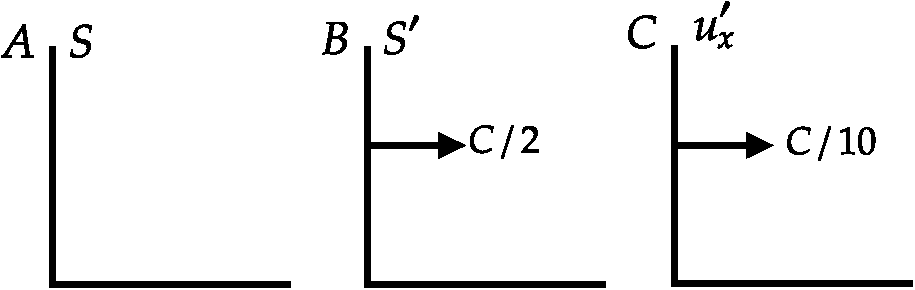
\includegraphics[height=3cm,width=9cm]{RM-2}
\end{figure}
\begin{align*}
v&=\frac{c}{2}, \quad u_{x}^{\prime}=\frac{c}{10}\\
u_{x}&=\frac{u_{x}^{\prime}+v}{1+\frac{u^{\prime} v_{x}}{c^{2}}}=\frac{4 c}{7}
\end{align*}
So the correct answer is \textbf{Option (B)}
\end{answer}
	\item A light signal travels from a point $A$ to a point $B$, both within a glass slab that is moving with uniform velocity (in the same direction as the light) with speed $0.3 c$ with respect to an external observer. If the refractive index of the slab is $1.5$, then the observer will measure the speed of the signal as
{	\exyear{NET/JRF(DEC-2017)}}
\begin{tasks}(4)
\task[\textbf{A.}] $0.67 c$
\task[\textbf{B.}]  $0.81 c$
\task[\textbf{C.}] $0.97 c$
\task[\textbf{D.}] $c$
\end{tasks}
\begin{answer}$\left. \right. $
\begin{figure}[H]
	\centering
	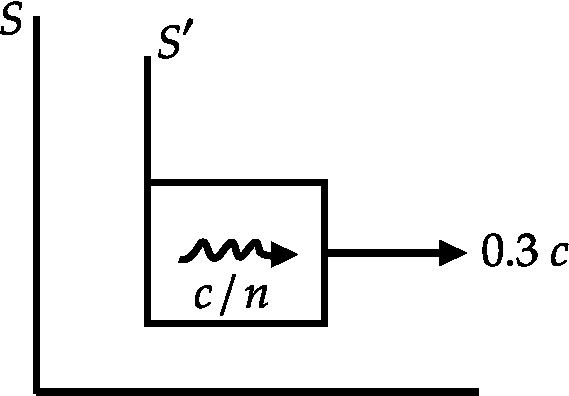
\includegraphics[height=3.5cm,width=5cm]{RM-1}
\end{figure}
\begin{align*}
v&=0.3 c\\
u_{x}^{\prime}&=\frac{c}{n} n=1.5\\
u_{x}&=\frac{u_{x}^{\prime}+v}{1+\frac{u_{x} v}{c^{2}}}=\frac{0.3 c+\frac{c}{n}}{1+\frac{c}{n} \cdot \frac{0.3 c}{c^{2}}}\\
u_{x}&=0.81 c
\end{align*}
So the correct answer is \textbf{Option (B)}
\end{answer}
	\item Consider a radioactive nucleus that is travelling at a speed $\frac{c}{2}$ with respect to the lab frame. It emits $\gamma$-rays of frequency $v_{0}$ in its rest frame. There is a stationary detector, (which is not on the path of the nucleus) in the lab. If a $\gamma$-ray photon is emitted when the nucleus is closest to the detector, its observed frequency at the detector is
{	\exyear{NET/JRF(DEC-2016)}}
\begin{tasks}(4)
\task[\textbf{A.}]  $\frac{\sqrt{3}}{2} v_{0}$
\task[\textbf{B.}] $\frac{1}{\sqrt{3}} v_{0}$
\task[\textbf{C.}] $\frac{1}{\sqrt{2}} v_{0}$
\task[\textbf{D.}] $\sqrt{\frac{2}{3}} v_{0}$
\end{tasks}
\begin{answer}
\begin{align*}
v&=v_{0} \sqrt{1-\frac{v^{2}}{c^{2}}}\quad \quad
\text{(If detector is not in the path at nucleus)}\\
v&=v_{0} \sqrt{1-\frac{1}{4}}=v_{0} \frac{\sqrt{3}}{2}
\end{align*}
So the correct answer is \textbf{Option (A)}
\end{answer}
	\item What is proper time interval between the occurrence of two events if in one inertial frame events are separated by $7.5 \times 10^{8} \mathrm{~m}$ and occur $6.5 \mathrm{~s}$ apart?
{	\exyear{NET/JRF(JUNE-2012)}}
\begin{tasks}(4)
\task[\textbf{A.}] $6.50 s$
\task[\textbf{B.}] $6.00 s$
\task[\textbf{C.}] $5.75 s$
\task[\textbf{D.}] 
\end{tasks}
\begin{answer}
\begin{align*}
\intertext{Proper time interval}
\Delta t&=\sqrt{\left(\Delta t^{\prime}\right)^{2}-\frac{r^{2}}{c^{2}}}=\sqrt{(6.5)^{2}-\left(\frac{7.5}{3}\right)^{2}}=6 \mathrm{sec}
\end{align*}
\end{answer}
	\item Let $v, p$ and $E$ denote the speed, the magnitude of the momentum, and the energy of a free particle of rest mass $m$. Then
	{NET/JRF (DEC-2012)}
	 \begin{tasks}(2)
		\task[\textbf{a.}]$\frac{d E}{d P}=c$ constant
		\task[\textbf{b.}] $p=m v$
		\task[\textbf{c.}]$v=\frac{c p}{\sqrt{p^{2}+m^{2} c^{2}}}$
		\task[\textbf{d.}] $E=m c^{2}$
	\end{tasks}
\begin{answer}
	\begin{align*}
	p&=m^{\prime} v=\frac{m v}{\sqrt{1-\frac{v^{2}}{c^{2}}}} \Rightarrow p^{2}=\frac{m^{2} v^{2}}{1-\frac{v^{2}}{c^{2}}} \Rightarrow m^{2} v^{2}=p^{2}-\frac{p^{2} v^{2}}{c^{2}}, m \rightarrow \text { rest mass energy }\\
	\Rightarrow v^{2}\left(m^{2}+\frac{p^{2}}{c^{2}}\right)&=p^{2} \Rightarrow v^{2}=\frac{p^{2}}{\frac{m^{2} c^{2}+p^{2}}{c^{2}}} \Rightarrow v=\frac{p c}{\sqrt{p^{2}+m^{2} c^{2}}}
	\end{align*}
	So the correct answer is \textbf{Option (c)}
\end{answer}
	\item Consider the decay process $\tau^{-} \rightarrow \pi^{-}+v_{\tau}$ in the rest frame of the $\tau^{-} .$The masses of the $\tau^{-}, \pi^{-}$and $v_{\tau}$ are $M_{\tau}, M_{\pi}$ and zero respectively.\\\\
	\textbf{A}. The energy of $\pi^{-}$is
{	\exyear{NET/JRF(JUNE-2011)}}
\begin{tasks}(4)
\task[\textbf{A.}] $\frac{\left(M_{\tau}^{2}-M_{\pi}^{2}\right) c^{2}}{2 M_{\tau}}$
\task[\textbf{B.}] $\frac{\left(M_{\tau}^{2}+M_{\pi}^{2}\right) c^{2}}{2 M_{\tau}}$
\task[\textbf{C.}] $\left(M_{\tau}-M_{\pi}\right) c^{2}$
\task[\textbf{D.}] $\sqrt{M_{\tau} M_{\pi}} c^{2}$
\end{tasks}
\begin{answer}
\begin{align*}
\tau^{-} \rightarrow \pi^{-}+v_{\tau}&\\
\text{From conservation of energy }\mathrm{M}_{\tau} \mathrm{c}^{2}&=\mathrm{E}_{\pi}+\mathrm{E}_{\mathrm{v}}
\intertext{$E_{\pi}^{2}=p^{2} c^{2}+M_{\pi}^{2} c^{4}$ and $E_{v}^{2}=p^{2} c^{2}$ since momentum of $\pi^{-}$and $v_{\tau}$ is same.}
M_{\tau} c^{2}&=E_{\pi}+E_{v}, M_{\pi}^{2} c^{4}\\&=E_{\pi}^{2}-E_{v}^{2} \Rightarrow E_{\pi}-E_{v}=\frac{M_{\pi}^{2} c^{4}}{M_{\tau} c^{2}}\\
E_{\pi}-E_{v}&=\frac{M_{\pi}^{2} c^{2}}{M_{\tau}}\text{ and }E_{\pi}+E_{v}\\&=M_{\tau} c^{2} \Rightarrow E_{\pi}=\frac{\left(M_{\tau}^{2}+M_{\pi}^{2}\right) c^{2}}{2 M_{\tau}}
\end{align*}
So the correct answer is \textbf{Option (B)}
\end{answer}
	\item The muon has mass $105 \mathrm{MeV} / \mathrm{c}^{2}$ and mean life time $2.2 \mu \mathrm{s}$ in its rest frame. The mean distance traversed by a muon of energy $315 \mathrm{MeV}$ before decaying is approximately,
{	\exyear{NET/JRF(DEC-2012)}}
\begin{tasks}(4)
\task[\textbf{A.}] $3 \times 10^{5} \mathrm{~km}$
\task[\textbf{B.}] $2.2 \mathrm{~cm}$
\task[\textbf{C.}] $6.6 \mu \mathrm{m}$
\task[\textbf{D.}] $1.98 \mathrm{~km}$
\end{tasks}
\begin{answer}
\begin{align*}
\text{Since }E&=315 \mathrm{MeV}\text{ and }m_{0}=105 \frac{\mathrm{MeV}}{c^{2}}.\\
E&=m c^{2} \Rightarrow E=\frac{m_{0} c^{2}}{\sqrt{1-\frac{v^{2}}{c^{2}}}} \Rightarrow 315\\&=\frac{m_{0} c^{2}}{\sqrt{1-\frac{v^{2}}{c^{2}}}} \Rightarrow 315=\frac{105}{\sqrt{1-\frac{v^{2}}{c^{2}}}} \Rightarrow v=0.94 c\\
\text{Now, }t&=\frac{t_{0}}{\sqrt{1-\frac{v^{2}}{c^{2}}}}, \quad t_{0}=2.2 \mu s \Rightarrow t\\&=\frac{2.2 \times 10^{-6}}{\sqrt{1-\frac{8}{9}}} \Rightarrow t=6.6 \mu \mathrm{s}
\intertext{Now the distance traversed by muon is $v t=0.94 c \times 6.6 \times 10^{-6}=1.86 \mathrm{~km}$.}
\end{align*}
So the correct answer is \textbf{Option (D)}
\end{answer}
	\item A constant force $F$ is applied to a relativistic particle of rest mass $m$. If the particle starts from rest at $t=0$, its speed after a time $t$ is
{	\exyear{NET/JRF(DEC-2011)}}
\begin{tasks}(4)
\task[\textbf{A.}] $F t / m$
\task[\textbf{B.}] $c \tanh \left(\frac{F t}{m c}\right)$
\task[\textbf{C.}] $c\left(1-e^{-F t / m c}\right)$
\task[\textbf{D.}] $\frac{F c t}{\sqrt{F^{2} t^{2}+m^{2} c^{2}}}$
\end{tasks}
\begin{answer}
\begin{align*}
\intertext{$\frac{d p}{d t}=F \Rightarrow p=F t+c$. At $t=0, p=0$ so, $c=0$}
\Rightarrow p&=F t \Rightarrow \frac{m u}{\sqrt{1-\frac{u^{2}}{c^{2}}}}=F t \Rightarrow u\\&=\frac{\left(\frac{F}{m}\right) t}{\sqrt{1+\left(\frac{F t}{m c}\right)^{2}}}=\frac{F c t}{\sqrt{F^{2} t^{2}+m^{2} c^{2}}}
\end{align*}
So the correct answer is \textbf{Option (D)}
\end{answer}
	\item For a particle of energy $E$ and momentum $p$ (in a frame $F$ ), the rapidity $y$ is defined as $y=\frac{1}{2} \ln \left(\frac{E+p_{3} c}{E-p_{3} c}\right) .$ In a frame $F^{\prime}$ moving with velocity $v=(0,0, \beta c)$ with respect to $F$, the rapidity $y^{\prime}$ will be
{	\exyear{NET/JRF(JUNE-2016)}}
\begin{tasks}(2)
\task[\textbf{A.}] $y^{\prime}=y+\frac{1}{2} \ln \left(1-\beta^{2}\right)$
\task[\textbf{B.}] $y^{\prime}=y-\frac{1}{2} \ln \left(\frac{1+\beta}{1-\beta}\right)$
\task[\textbf{C.}]  $y^{\prime}=y+\ln \left(\frac{1+\beta}{1-\beta}\right)$
\task[\textbf{D.}] $y^{\prime}=y+2 \ln \left(\frac{1+\beta}{1-\beta}\right)$
\end{tasks}
\begin{answer}
\begin{align*}
y&=\frac{1}{2} \ln \left(\frac{E+p_{3} c}{E-p_{3} c}\right)\\
\text{Then }y^{\prime}&=\frac{1}{2} \ln \left(\frac{E^{\prime}+p_{3}^{\prime} c}{E^{\prime}-p_{3}^{\prime} c}\right)\\
\text{	Where }p_{3}^{\prime}&=\gamma\left(p_{3}-v\left(\frac{E}{c^{2}}\right)\right) \quad \quad E^{\prime}=\gamma\left(E-v p_{3}\right)
\intertext{Put the value of $p_{3}^{\prime}$ and $E^{\prime}$ one will get $y^{\prime}=\frac{1}{2} \ln \left(\frac{\left(E+p_{3} c\right)-\frac{v}{c}\left(E+p_{3} c\right)}{\left(E-p_{3} c\right)+\frac{v}{c}\left(E-p_{3} c\right)}\right)$}
\frac{1}{2} \ln \left(\frac{\left(E+p_{3} c\right)(1-\beta)}{\left(E-p_{3} c\right)(1+\beta)}\right) &\Rightarrow \frac{1}{2} \ln \left(\frac{\left(E+p_{3} c\right)}{\left(E-p_{3} c\right)}\right)+\frac{1}{2} \ln \left(\frac{1-\beta}{1+\beta}\right)\\
y+\frac{1}{2} \ln \left(\frac{1-\beta}{1+\beta}\right) &\Rightarrow y-\frac{1}{2} \ln \left(\frac{1+\beta}{1-\beta}\right)
\end{align*}
So the correct answer is \textbf{Option (B)}
\end{answer}
	\item Which of the following questions is Lorentz invariant?
{	NET/JRF-(JUNE-2012)}
 \begin{tasks}(2)
	\task[\textbf{a.}]$|\vec{E} \times \vec{B}|^{2}$
	\task[\textbf{b.}] $|\vec{E}|^{2}-|\vec{B}|^{2}$
	\task[\textbf{c.}]$|\vec{E}|^{2}+|\vec{B}|^{2}$
	\task[\textbf{d.}] $|\vec{E}|^{2}|\vec{B}|^{2}$
\end{tasks}
\begin{answer}
	So the correct answer is \textbf{Option (b)}
\end{answer}
\item In an inertial frame $S$, the magnetic vector potential in a region of space is given by $\vec{A}=a z \hat{i}$ (where $a$ is a constant) and the scalar potential is zero. The electric and magnetic fields seen by an inertial observer moving with a velocity $v \hat{i}$ with respect to $S$, are, respectively [In the following $\gamma=\frac{1}{\sqrt{1-\frac{v^{2}}{c^{2}}}}$ ] 
{NET/JRF-(DEC-2017)}
 \begin{tasks}(2)
	\task[\textbf{a.}]0 and $\gamma a \hat{j}$
	\task[\textbf{b.}]$-v a \hat{k}$ and $\gamma a \hat{i}$
	\task[\textbf{c.}]$v \gamma a \hat{k}$ and $v \gamma a \hat{j}$
	\task[\textbf{d.}] $v \gamma a \hat{k}$ and $\gamma a \hat{j}$
\end{tasks}
\begin{answer}
	\begin{align*}
	E_{x}&=E_{x}^{\prime}, E_{y}=\gamma\left(E_{y}^{\prime}+v B_{z}^{\prime}\right) \text { and } E_{z}=\gamma\left(E_{z}^{\prime}-v B_{y}^{\prime}\right)\\
	B_{x}&=B_{x}^{\prime}, B_{y}=\gamma\left(B_{y}^{\prime}-\frac{v}{c^{2}} E_{z}^{\prime}\right) \text { and } B_{z}=\gamma\left(B_{z}^{\prime}+\frac{v}{c^{2}} E_{y}^{\prime}\right)\\
	\vec{E}^{\prime}&=-\vec{\nabla} V^{\prime}-\frac{\partial \vec{A}^{\prime}}{\partial t}=0, \vec{B}^{\prime}=\vec{\nabla} \times \vec{A}^{\prime}=a \hat{j}\\
	E_{x}&=0, E_{y}=\gamma(0-v \times 0)=0, E_{z}=\gamma(0+v a)=\gamma v a\\
	\text { (replace }& v \text { by }-v) \Rightarrow \vec{E}=v \gamma a \hat{z}\\
	B_{x}&=0, B_{y}=\gamma\left(a+\frac{v}{c^{2}} \times 0\right)=\gamma a, B_{z}=\gamma\left(0-\frac{v}{c^{2}} \times 0\right)=0\\
	\Rightarrow \vec{B}&=\gamma a \hat{j}
	\end{align*}
	So the correct answer is \textbf{Option (d)}
\end{answer}
\item The value of the electric and magnetic fields in a particular reference frame (in Gaussian units) are $E=3 \hat{x}+4 \hat{y}$ and $B=3 \hat{z}$ respectively. An inertial observer moving with respect to this frame measures the magnitude of the electric field to be $\left|E^{\prime}\right|=4$. The magnitude of the magnetic field $\left|B^{\prime}\right|$ measured by him is
{NET/JRF-(JUNE-2016)}
 \begin{tasks}(2)
	\task[\textbf{a.}]5
	\task[\textbf{b.}]9
	\task[\textbf{c.}]0
	\task[\textbf{d.}] 1
\end{tasks}
\begin{answer}
	\begin{align*}
	\because E^{2}-B^{2}=E^{\prime 2}-B^{\prime 2}=\text { constant } \Rightarrow(9+16)-9=16-B^{\prime 2} \Rightarrow B^{\prime}=0
	\end{align*}
		So the correct answer is \textbf{Option (c)}
\end{answer}
\item A inertial observer $A$ at rest measures the electric and magnetic field $E=(\alpha, 0,0)$ and $B=(\alpha, 0,2 \alpha)$ in a region, where a is a constant. Another inertial observer $B$, moving with a constant velocity with respect to $A$, measures the fields as $E^{\prime}=\left(E_{x}^{\prime}, \alpha, 0\right)$ and $B^{\prime}=\left(\alpha, B_{y}^{\prime}, \alpha\right)$. Then in units $c=1, E_{x}^{\prime}$ and $B_{y}^{\prime}$ are given, respectively, by
NET/JRF (June-2019)
 \begin{tasks}(2)
	\task[\textbf{a.}]$-2 \alpha$ and $\alpha$
	\task[\textbf{b.}] $2 \alpha$ and $-\alpha$
	\task[\textbf{c.}] $\alpha$ and $-2 \alpha$
	\task[\textbf{d.}] $-\alpha$ and $2 \alpha$
\end{tasks}
\begin{answer}
	\begin{align*}
	\text { From } S\\
	E . B &\text { is invariant and } E^{2}-B^{2} \text { is invariant }\\
	E_{x}^{\prime 2}-B_{y}^{\prime 2}&=-3 \alpha^{2}\\
	E_{x}^{\prime}+B_{y}^{\prime}&=\alpha \text { (Solving these two equation) }\\
	E_{x}^{\prime}&=-\alpha, \quad B_{y}^{\prime}=2 \alpha\\
	\text { Option }& 4 \text { is correct. }
	\end{align*}
			So the correct answer is \textbf{Option (c)}
\end{answer}
\item A heavy particle of rest mass $M$ while moving along the positive $z$ - direction, decays into two identical light particles with rest mass $m$ (where $M>2 m$ ). The maximum value of the momentum that any one of the lighter particles can have in a direction perpendicular to the $z$ direction, is
{\exyear{NET/JRF(JUNE-2020)}}
\begin{tasks}(4)
\task[\textbf{A.}]  $\frac{1}{2} C \sqrt{M^{2}-4 m^{2}}$
\task[\textbf{B.}] $\frac{1}{2} C \sqrt{M^{2}-2 m^{2}}$
\task[\textbf{C.}] $C \sqrt{M^{2}-4 m^{2}}$
\task[\textbf{D.}]  $\frac{1}{2} M C$
\end{tasks}
\begin{answer}$\left. \right. $
\begin{figure}[H]
	\centering
	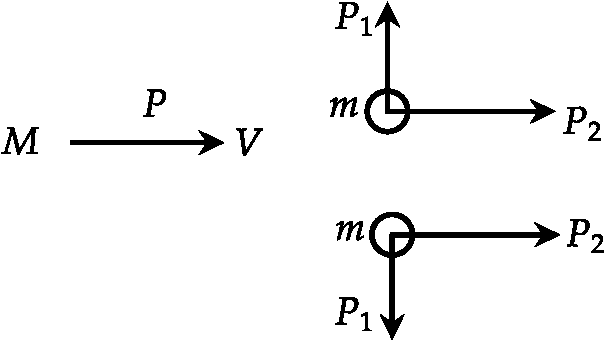
\includegraphics[height=3cm,width=5cm]{RM-4}
\end{figure}
\begin{align*}
\intertext{Let $P$ be the momentum of heavy mass $M .$ And let $P_{1}$ be the momentum of the light particles of mass $m$ in the direction perpendicular to $z$ and $P_{2}$ be the momentum in $z$-direction. According to conservation of momentum,}
\text{Momentum of mass }M, P&=P_{2}+P_{2}=2 P_{2} \Rightarrow P_{2}=P / 2\\
\text{Energy of }\operatorname{mass} M, E&=\sqrt{P^{2} c^{2}+M^{2} c^{4}}\\
\text{Momentum of a mass }m,=\sqrt{P_{1}^{2}+P_{2}^{2}}&=\sqrt{P_{1}^{2}+\frac{P^{2}}{4}}\\
\text{	Energy of mass }m, E_{1}^{2}&=\left(P_{1}^{2}+\frac{P^{2}}{4}\right) c^{2}+m^{2} c^{4}\\
\text{As energy is conserved }E&=E_{1}+E_{2}=2 E_{1} \Rightarrow E_{1}=\frac{E}{2}\qquad \because E_{1}=E_{2}\\
\text{Thus }E_{1}^{2}&=\frac{E^{2}}{4}=\left(P_{1}^{2}+\frac{P^{2}}{4}\right) c^{2}+m^{2} c^{4} \\&\Rightarrow 4\left(P_{1}^{2}+\frac{P^{2}}{4}\right) c^{2}+4 m^{2} c^{4}=P^{2} c^{2}+M^{2} c^{4}\\
4 P_{1}^{2} c^{2}+P^{2} c^{2}+4 m^{2} c^{4}&=P^{2} c^{2}+M^{2} c^{4} \Rightarrow 4 P_{1}^{2} c^{2}+4 m^{2} c^{4}\\&=M^{2} c^{4} \Rightarrow 4 P_{1}^{2}=M^{2} c^{2}-4 m^{2} c^{2}\\
P_{1}^{2}&=\frac{c^{2}}{4}\left(M^{2}-4 m^{2}\right) \Rightarrow P_{1}=\frac{c}{2} \sqrt{M^{2}-4 m^{2}}
\end{align*}
So the correct answer is \textbf{Option (A)}
\end{answer}
\end{enumerate}